%!TEX root = ..\ms-thesis.tex
\chapter{Literature Review} \label{ch:literature-review}

\section{Cast Heat-Resistant Stainless Steels}
Cast heat-resistant stainless steels can be broadly considered as the families of cast alloys which are designed for sustained elevated temperature service above \SmartUnit{fahrenheit=1200}~\cite{blair_cast_stainless_1990}.  The compositions of heat-resistant stainless steels primarily fall within the categories of Fe-Cr, Fe-Cr-Ni, and Fe-Ni-Cr alloys, with varying chromium and nickel contents, e.g. as shown in Figure~\ref{fig:aci-alloy-designations} for a number of alloy designations assigned by the Alloy Casting Institute. The chromium and nickel contents influence the resulting microstructure, with the Fe-Cr grades (e.g.~the HA series) being predominantly ferritic~\cite{davis_metallurgy_1994}. Fe-Cr-Ni grades are either austenitic-ferritic (duplex) or fully austenitic depending on the particular composition and balance of chromium and nickel, while the Fe-Ni-Cr alloys are fully austenitic. Due to their significant chromium content which results in a stable oxide layer at the surface, heat-resistant alloys exhibit good-to-excellent resistance to corrosion and oxidation in high temperature environments (e.g.~carburizing, nitriding)~\cite{davis_metallurgy_1994}. High temperature (creep) strength varies according to microstructure, with the ferritic Fe-Cr alloys exhibiting comparatively lower strength at elevated temperatures~\cite{avery_cast_1969} and thus are typically confined to applications requiring high-temperature corrosion resistance under moderate loading~\cite{davis_metallurgy_1994}; the fully austenitic heat-resistant stainless steels exhibit superior high temperature strength. The principal mechanism providing high temperature strength in heat-resistant stainless steels is the uniform precipitation of fine secondary carbides throughout the matrix~\cite{avery_cast_1969,davis_metallurgy_1994}. 

% Metallurgy
% Source of high temperature strength
% Fine dispersion of carbides/nitrides in matrix (avery)
% GB NbC carbides reduce GB sliding (wadsworth 1976)

\begin{figure}
\centering
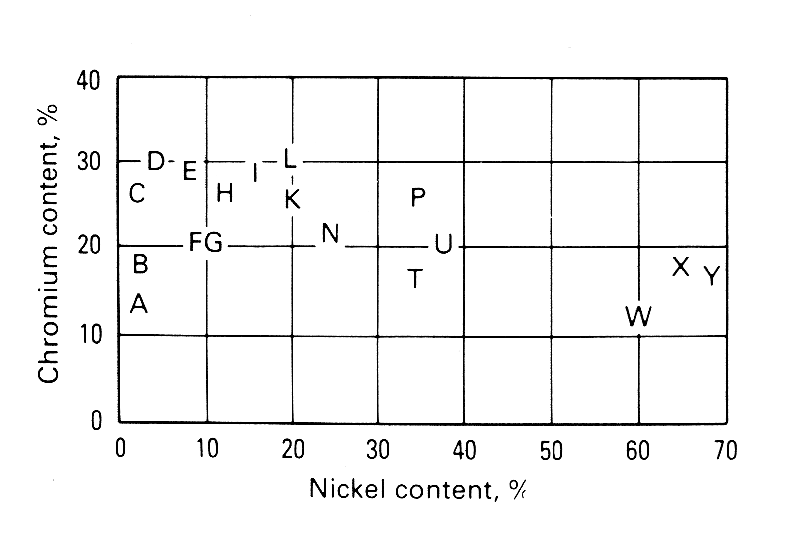
\includegraphics[width=3in]{figures/aci-designation.png}
\caption[Diagram indicating chromium and nickel contents of various cast stainless steel compositions according to the letter designations of the Alloy Casting Institute.]{Diagram indicating chromium and nickel contents of various cast stainless steel compositions using the letter designations of the Alloy Casting Institute. Each letter is combined with a “C” prefix for corrosion-resisting alloys or a “H” for heat-resisting alloys (e.g. the designation “HT“ denotes a heat-resistant alloy with 16 wt\% Cr, 35 wt\% Ni). From \citet{blair_cast_stainless_1990}.}
\label{fig:aci-alloy-designations}
\end{figure}

\subsection{Effects of Alloying Elements}
Chromium (Cr) is a principal alloying element in heat-resistant stainless steels, with typical Cr contents in the range of \numrange[range-phrase=--]{10}{30}\% as shown in the summary of various alloy designations in Figure~\ref{fig:aci-alloy-designations}. Chromium is added primarily for high temperature oxidation resistance which originates from the formation of a stable, adherent surface layer of chromium oxide~\cite{kane_evolution_1991}. Chromium is a strong ferrite stabilizer~\cite{folkhard_welding_1988} and thus in alloys where a fully austenitic structure is desired but which may be lean in austenite-stabilizing elements (e.g. the HH series), the Cr content must be balanced carefully~\cite{avery_cast_1969}. Chromium also combines with carbon to form a variety of carbides, with the (Fe,Cr)$_\textnormal{23}$C$_\textnormal{6}$ complex carbide being the primary type in heat-resistant stainless steels~\cite{sourmail_precipitation_2001}. Although precipitation of Cr carbides contributes to creep strength, Cr carbides are less stable at higher temperature ranges and have a tendency to coarsen, reducing their strengthening effect~\cite{avery_cast_1969}.

In combination with chromium, nickel (Ni) constitutes the other primary alloying element in heat-resistant stainless steels. Nickel content in heat-resistant alloys varies over a wide range, \numrange[range-phrase=--]{1}{60}\% (Figure~\ref{fig:aci-alloy-designations}). Nickel is a strong austenite stabilizer~\cite{folkhard_welding_1988} and thus sufficient addition of Ni permits fully austenitic microstructures at room temperature. Nickel is also beneficial for resistance to high temperature oxidation and carburization by promoting a stable chromium oxide layer, and thus alloys intended for higher temperature service utilize higher nickel contents~\cite{kane_evolution_1991}.

The primary function of niobium (Nb) additions in heat-resistant alloys is to increase the high-temperature creep strength. Niobium combines preferentially with carbon to form niobium carbides (NbC), which are more stable at elevated temperatures than chromium carbides with a lower tendency for coarsening~\cite{keown_niobium_1981}. In cast alloys, NbC forms as a eutectic carbide along the interdendritic boundaries~\cite{davis_metallurgy_1994} which contributes to improved creep performance by inhibiting grain boundary sliding~\cite{de_almeida_soares_niobium_1992-1}. Niobium carbide also forms as fine intradendritic carbides within the matrix~\cite{chen_characterisation_2004}, both in as-cast condition and after high temperature exposure. High niobium levels (well above the stoichiometric amount required for formation of NbC) are associated with reduced oxidation resistance~\cite{collins_effect_1980}.

Silicon (Si) is added as an intentional alloying element in heat-resistant stainless steels as a deoxidizer (typical steel-making practice) and also for the purpose of increasing the high temperature oxidation resistance~\cite{kane_evolution_1991} by improving the adhesion of the protective chromium oxide layer that forms on the surface of heat-resistant alloys. However, it has been observed that increasing silicon content is correlated with a reduction in creep strength in heat-resistant alloys~\cite{avery_cast_1969}. Additionally, the tendencies for formation of embrittling sigma phase and for formation of Ni-Nb-Si phases (Ni-Nb silicide or G-phase) during high temperature exposure both increase as the silicon content increases~\cite{pedro_ibanez_effects_1993,davis_metallurgy_1994}. In cast alloys, silicon is also added to obtain good fluidity of the molten metal for improved casting quality~\cite{blair_cast_stainless_1990}.

\subsection{High Temperature Behavior}
During exposure to an elevated temperature environment, cast heat-resistant stainless steels experience a number of microstructural changes. Starting from the as-cast condition, high temperature exposure leads to the precipitation of carbides in the austenitic matrix, due to the fact that the as-cast material may retain significant carbon in solid solution~\cite{avery_cast_1969}. The degree of precipitation is dependent on the carbon content, with higher carbon alloys exhibiting a greater extent of carbide precipitation. Additionally, the morphology of the carbides is dependent on the temperature range which initiates precipitation (at the beginning of service), e.g. initial exposure at \SmartUnit{fahrenheit=1200} will precipitate finer carbides than exposure at \SmartUnit{fahrenheit=1600}~\cite{avery_cast_1969}. After longer duration exposure, particularly at higher temperatures (e.g. \SmartUnit{fahrenheit=2000}), the carbides in the matrix will coarsen with a consequent detrimental effect on creep strength~\cite{avery_cast_1969}.

% Carbide precipitation
% Other intermetallic phases such as sigma and z-phase (not well characterized)
% Weldability??

In addition to carbide precipitation and/or coarsening, high temperature exposure can result in the formation of other intermetallic phases, depending on the chemical composition.  Particularly in fully or partially ferritic heat-resistant stainless steels, the intermetallic constituent sigma phase (FeCr) can form which embrittles stainless steels and reduces creep strength when located on grain boundaries~\cite{sourmail_precipitation_2001,avery_cast_1969}. Of particular concern in the niobium-alloyed heat-resistant stainless steels is the potential formation of silicide phases after elevated temperature exposure; one such constituent is G-phase, which is usually associated with a nickel and niobium-rich composition (Ni$_\textnormal{16}$Nb$_\textnormal{6}$Si$_\textnormal{7}$)~\cite{sourmail_precipitation_2001}. The tendency for formation of G-phase increases with increasing silicon content~\cite{ecob_formation_1987,pedro_ibanez_effects_1993}. In cast 20Cr-32Ni-1Nb heat-resistant stainless steel (ASTM A351 Gr. CT15C), the formation of Ni-Nb-Si constituents has been frequently observed after service exposure in the range of \SIrange[range-phrase=--]{760}{850}{\degreeCelsius} (1400\,\textdegree{}F--1560\,\textdegree{}F). The formation of silicide phases in this alloy has been associated with reduced room temperature mechanical properties~\cite{hoffman_high_2000-1,shibasaki_experience_1994}, reduced creep strength~\cite{shibasaki_experience_1994}, and also with severe \gls{haz} cracking problems during repair welding~\cite{hoffman_weld_1998,knowles_service_2004}.

% CT15C
% Formation of Ni-Nb silicides which are correlated with reduced mechanical properties and weldability problems

\section{Liquation Cracking} \label{sec:liquation-cracking}
Liquation cracking is a type of weld-related “hot” cracking\footnote{“Hot” cracking occurs at high temperatures during welding, as opposed to “cold” cracking which occurs at or near ambient temperature (e.g. hydrogen related cracking).} which is associated with the formation\footnote{In contrast to solidification cracking (another form of hot cracking) in the weld deposit, wherein cracking is associated with liquid films \emph{remaining} along the boundaries at the terminal stages of solidification.} of liquid films along grain boundaries in the \gls{haz}, immediately adjacent to the fusion line, as a result of a high temperature excursion during a welding thermal cycle ~\cite{lippold_welding_2014}. Liquation cracking occurs at this location because the region of the \gls{haz} immediately adjacent to the fusion line is the region which is subjected to the highest peak temperatures during welding. Although liquation cracking can occur both in the base metal \gls{haz} and in weld metal \gls{haz}s (in the case of reheated weld metal in multi-pass weldments), only the former will be discussed here. In common with other forms of hot cracking, \gls{haz} liquation cracking requires the simultaneous occurrence of two factors: a critical level of applied strain and a susceptible microstructure exhibiting limited ductility over a critical temperature range. The imposition of strain on the \gls{haz} is inherent to welding, either from mechanical restraint (e.g. arising from the weld geometry or from external fixturing) or from thermal contraction during the on-cooling portion of a welding thermal cycle. \citet{yeniscavich_correlation_1970} estimated the level of thermal strain in the \gls{haz} to be on the order of < 1\%, indicating that an \gls{haz} region must exhibit essentially zero ductility for cracking to occur. 

%Figure showing distribution of strain in the HAZ???

A condition of zero ductility in the \gls{haz} originates from the formation of liquid films along the grain boundaries in the \gls{haz}, since liquid films have very limited capability to support strain. Liquid along the grain boundaries can be formed from several sources by the high temperatures experienced in the \gls{haz} during welding. Segregation of impurity elements and/or alloying elements (in solid solution) will occur at grain boundaries, since these regions were the last to solidify during the initial casting process and thus will have an inherently lower melting temperature than the adjacent matrix. This is especially true of cast materials where the original dendritic structure has not been disrupted by subsequent working/forming operations (as would occur for wrought materials). Another potential source of liquation is low-melting point phases which preferentially form at grain boundaries (again, due to segregation). Finally, liquid can also be formed by the mechanism of constitutional liquation as developed by~\citet{pepe_effects_1967}. Constitutional liquation is a non-equilibrium phenomenon arising from the rapid heating rates typical of welding and can be explained in a simplified manner in relation to the schematic binary phase diagram shown in Figure~\ref{pepe-liquation-diagram}. For a nominal composition $C_0$ which exhibits a two-phase microstructure at low temperatures, during the heating portion of a welding thermal cycle the temperature will increase to the point ($T_3$) where the equilibrium phase diagram predicts a single phase region and thus the secondary phase constituent will begin to dissolve. However, due to the rapid heating rate associated with welding, insufficient time is available for complete dissolution of the secondary constituent before the temperature exceeds the local melting point, in the following manner. Because the dissolution of the secondary phase must proceed by diffusion, if the diffusion rate of solute away from the secondary phase is slow, dissolution will create a concentration gradient at the interface of the secondary phase and the surrounding matrix, wherein a region of the matrix enriched in solute will exist around the particle. As the temperature continues to increase rapidly during the heating portion of the thermal cycle, the temperature will eventually exceed the local melting temperature of the enriched region (e.g. above $T_e$) and liquid will form. It is important to point out that in this reaction, the temperature at which liquid begins to form is well below the solidus temperatures of both the secondary constituent and the bulk matrix composition. In the case where the secondary phase exists primarily along grain boundaries (or interdendritic boundaries in a cast material), constitutional liquation of the secondary phase will produce liquid along the boundaries and thereby establish the conditions for liquation cracking. Constitutional liquation of constituent particles in the \gls{haz} has been observed in a number of alloy systems, e.g. liquation of Ti-rich phases in Alloy 800~\cite{lippold_investigation_1983} and liquation of niobium carbide (NbC) in Inconel 718~\cite{radhakrishnan_phase_1991} and AISI 347~\cite{lee_weldability_1988}.

\begin{figure}
    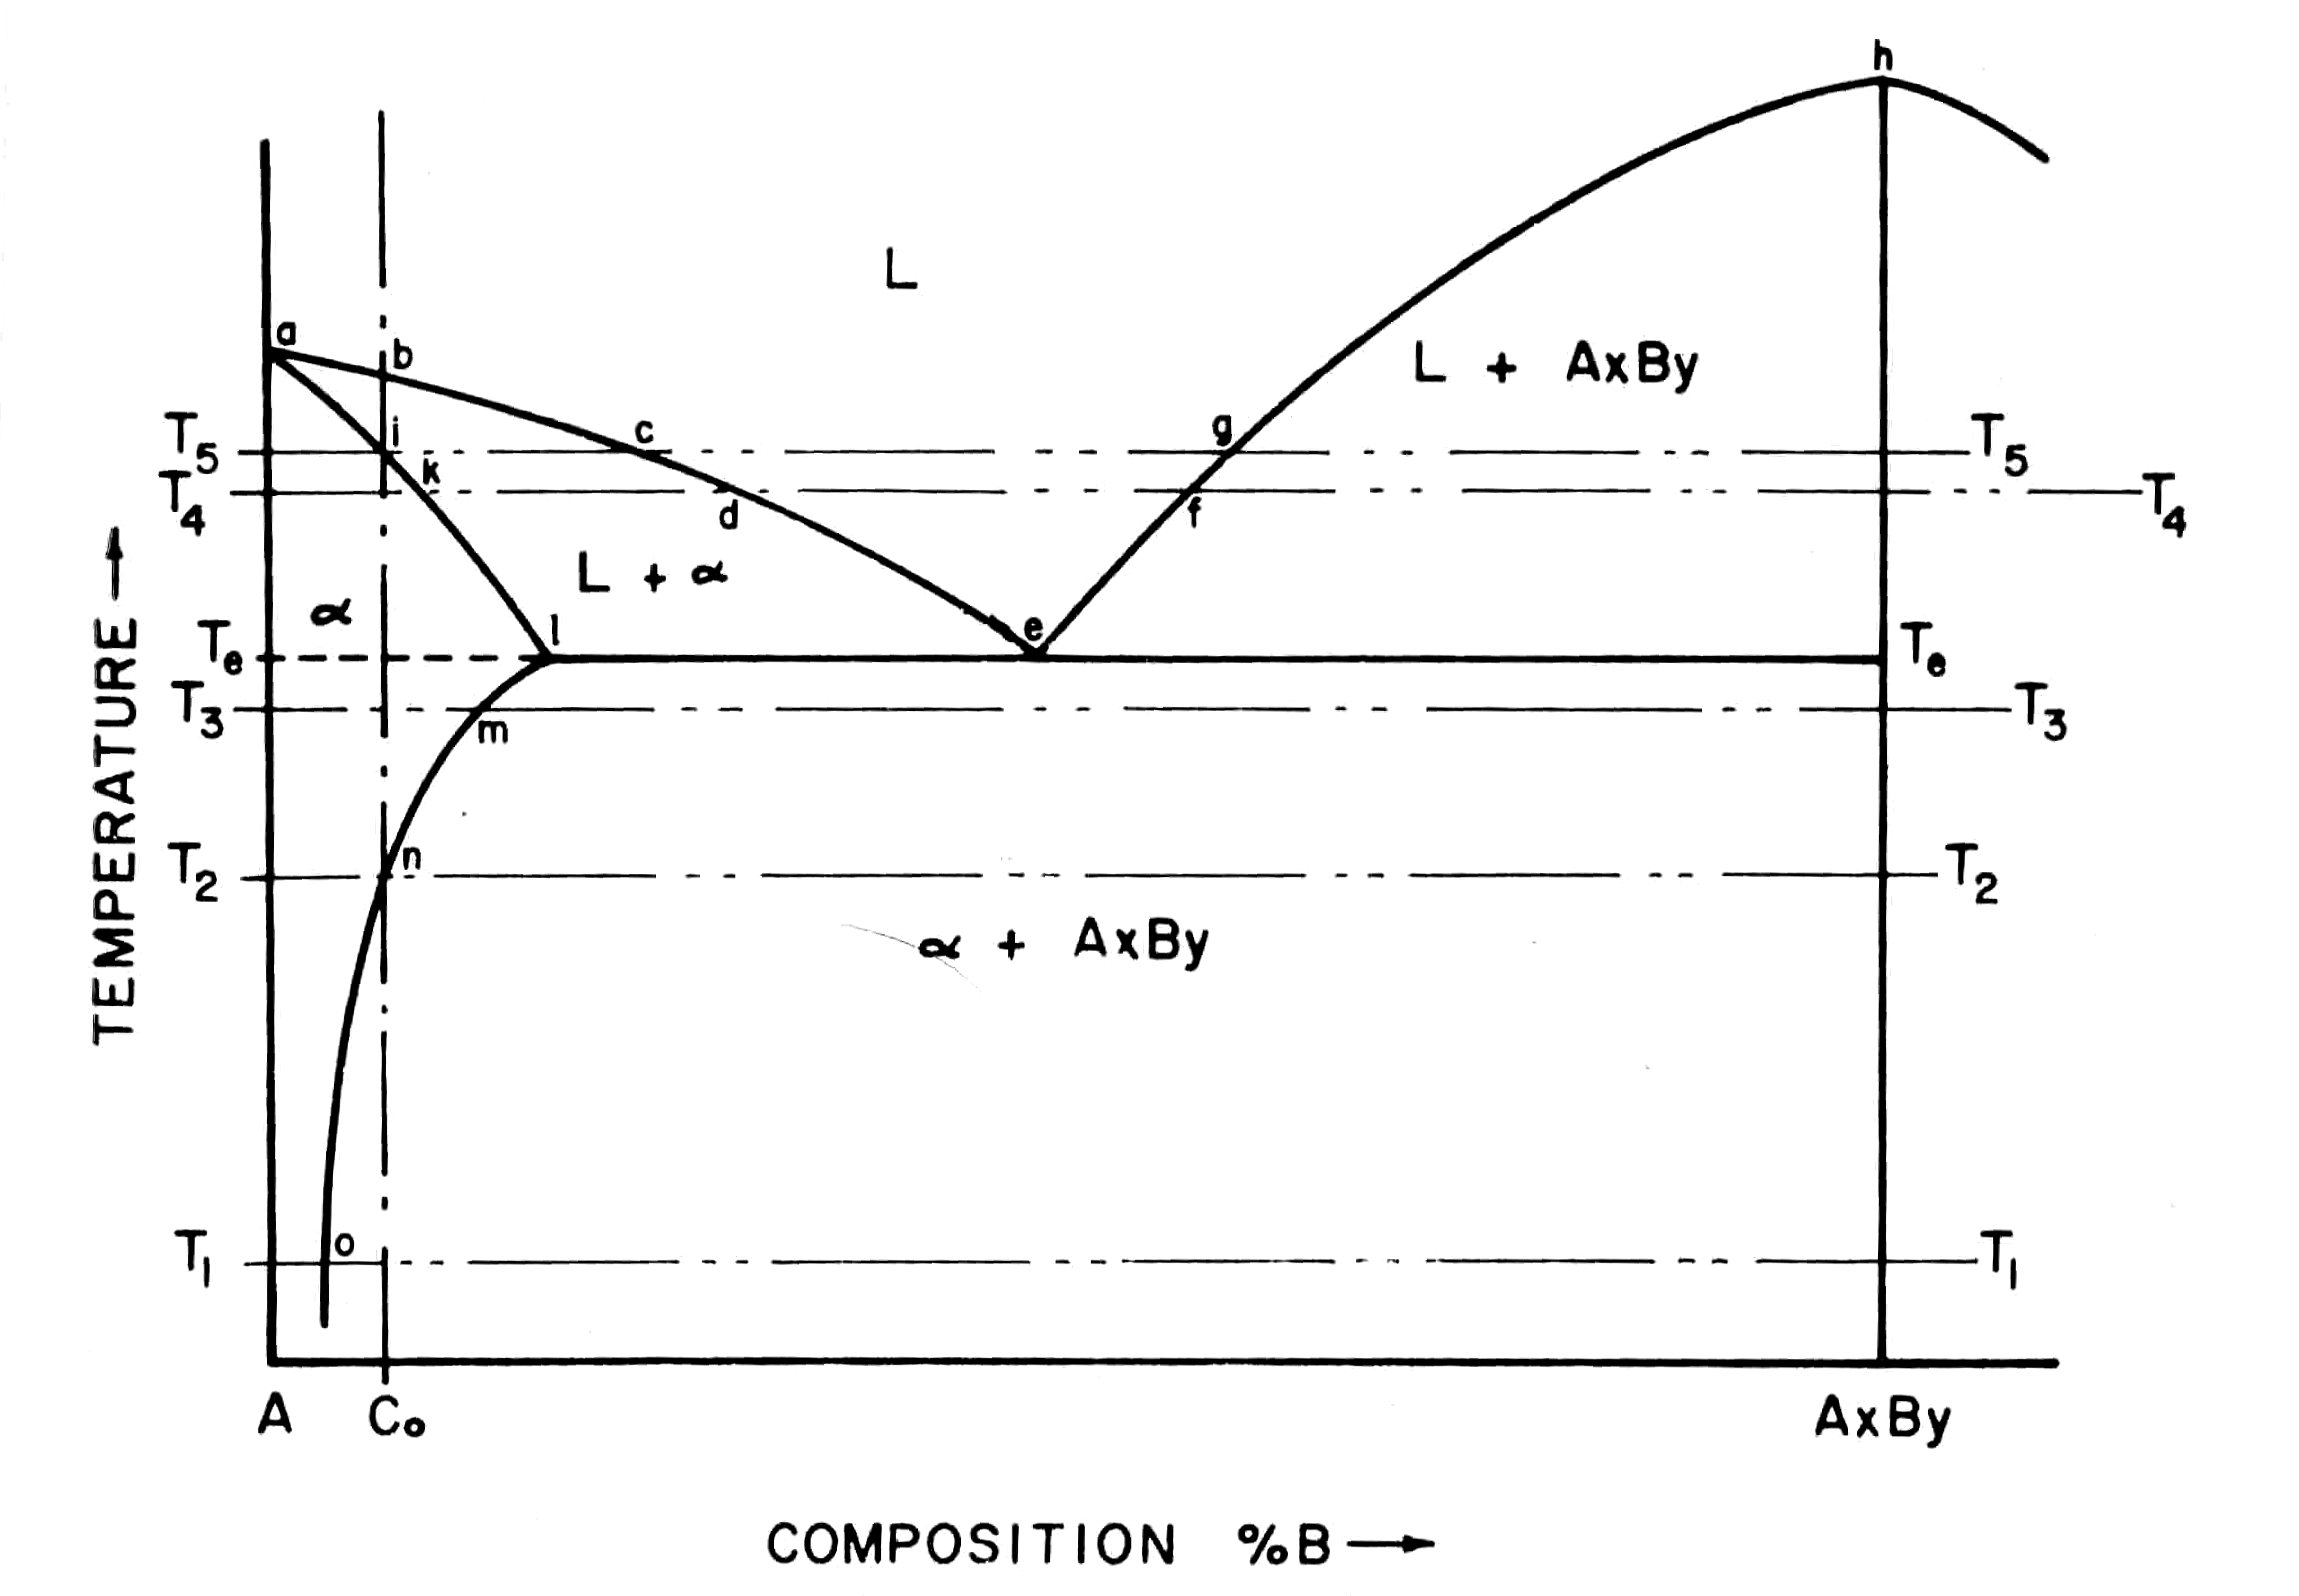
\includegraphics[width=6in]{figures/pepe-liquation-diagram.png}
    \caption{Illustration of a simple binary system in which constitutional liquation of the (AxBy) phase can occur under conditions of non-equilibrium heating (e.g. as would be typical of welding) to temperatures above $T_e$. From \citet{pepe_effects_1967}.}
    \label{pepe-liquation-diagram}
\end{figure}

% In general, explanations of liquation cracking phenomena in the \gls{haz} originate from weld metal hot cracking (i.e. solidification cracking) theories. 

% Liquation cracks vs hot cracks in PMZ of weld HAZ (show diagram)


\section{Weldability Evaluation} \label{sec:weldability-evaluation}

The term \emph{weldability} as defined by the American Welding Society corresponds to “the capacity of [a] material to be welded under the imposed fabrication conditions into a specific, suitably designed structure performing satisfactorily in the intended service“~\cite{aws_terms_2010}. Thus, the weldability of a material encompasses both the fabrication and in-service performance characteristics of a completed weldment. In order to evaluate these characteristics, \emph{weldability testing} is performed to ensure that a given combination of material, weld configuration/design, and welding parameters will result in a satisfactory weldment. A number of weldability tests to evaluate susceptibility to hot cracking and liquation cracking (described in Section~\ref{sec:liquation-cracking}) have been developed and are divided into two categories: self-restraint tests and externally-loaded tests~\cite{farrar_hot_2005}. As described in Section~\ref{sec:liquation-cracking}, liquation cracking (and hot cracking in general) essentially arises from the inability of a susceptible microstructure to accommodate strain over a particular critical temperature range. In self-restraint tests, the inherent restraint of the chosen weld configuration is used as the source of strain, while in externally-loaded tests, the strain is applied by an external device or instrument. Self-restraint tests are generally considered to be a qualitative, “go/no-go” type of test in contrast to externally-loaded tests which are designed to impose strain under controlled conditions and thus are a more quantitative evaluation method that is more sensitive to variables in materials or welding conditions~\cite{farrar_hot_2005}. Among externally-loaded tests for evaluating liquation cracking, two that are widely used are the Varestraint test~\cite{lundin_varestraint_1965} and the Gleeble\textregistered{} hot ductility test~\cite{nippes_investigation_1955}. The latter test method was utilized in the current study and a summary of the test method and associated evaluation criteria are described in the following sections.

% The requirements of an “ideal” weldability test include the following (DMIC report 165):

% \begin{compactenum}
% \item Direct correlation with actual fabrication or service
% \item High sensitivity to the effects of welding variables
% \item Good reproducibility of results
% \item Simplicity
% \item Economy in the use of materials
% \item Low cost
% \item Applicability to all welding processes
% \end{compactenum}


\subsection{The Hot Ductility Test}
The origin of the hot ductility test can be traced back to work performed by \citet{nippes_cooling_1949} on the measurement of the actual time-temperature history (“thermal cycle”) experienced in the \gls{haz} of various alloys during welding.  Using this data as a foundation, \citet{nippes_development_1949} developed a device, the “Gleeble,” capable of reproducing a given thermal cycle by resistively heating a sample and controlling the temperature as a function of time using an attached fine-wire thermocouple. This technique enabled the duplication of a specific region of the \gls{haz} in a macroscopically-sized sample suitable for mechanical testing.  The capabilities of the machine were expanded by adding a loading system which permitted the sample to be deformed or fractured at any point in the thermal cycle.  This capability of the Gleeble\textregistered{} was put to use in the development of the hot ductility test~\cite{nippes_investigation_1955}, in which the ductility of a particular alloy (in terms of percent reduction in cross-sectional area) is determined at various time-temperature points in the thermal cycle.  The hot ductility is normally determined in two distinct modes: “on-heating” and “on-cooling.”  Tests to determine “on-heating” hot ductility are performed during the initial portion of the thermal cycle where the sample is heated rapidly toward the peak temperature (see Figure~\ref{subfig:on-heating-schematic}).  On-heating tests are typically performed at sequentially higher temperatures approaching the calculated \gls{haz} peak temperature (usually in the vicinity of 2400\textdegree{}F) until a test temperature is reached where the measured on-heating ductility drops to zero (0\%~RA).  This temperature is designated the \gls{zdt}.  Once the \gls{zdt} has been determined, “on-cooling” hot ductility tests are performed in the portion of the thermal cycle where the sample temperature is decreasing after exposure to a peak temperature corresponding to the \gls{zdt} (see Figure~\ref{subfig:on-cooling-schematic}).  As will be discussed later, the on-cooling ductility behavior is considered the most indicative factor regarding a material’s susceptibility to hot cracking.  Figure~\ref{fig:schematic-hot-ductility-curves} shows schematic examples of the types of curves which can be constructed using the data obtained (\%RA vs. test temperature) from the on-heating and on-cooling hot ductility tests just described; important features of these curves are labeled in the plot and will be discussed in more detail in the following section. Further details regarding the history and development of the Gleeble, including references to other development papers not 
\begin{figure}
    \centering
    \subfloat[On-heating hot ductility testing]{\label{subfig:on-heating-schematic}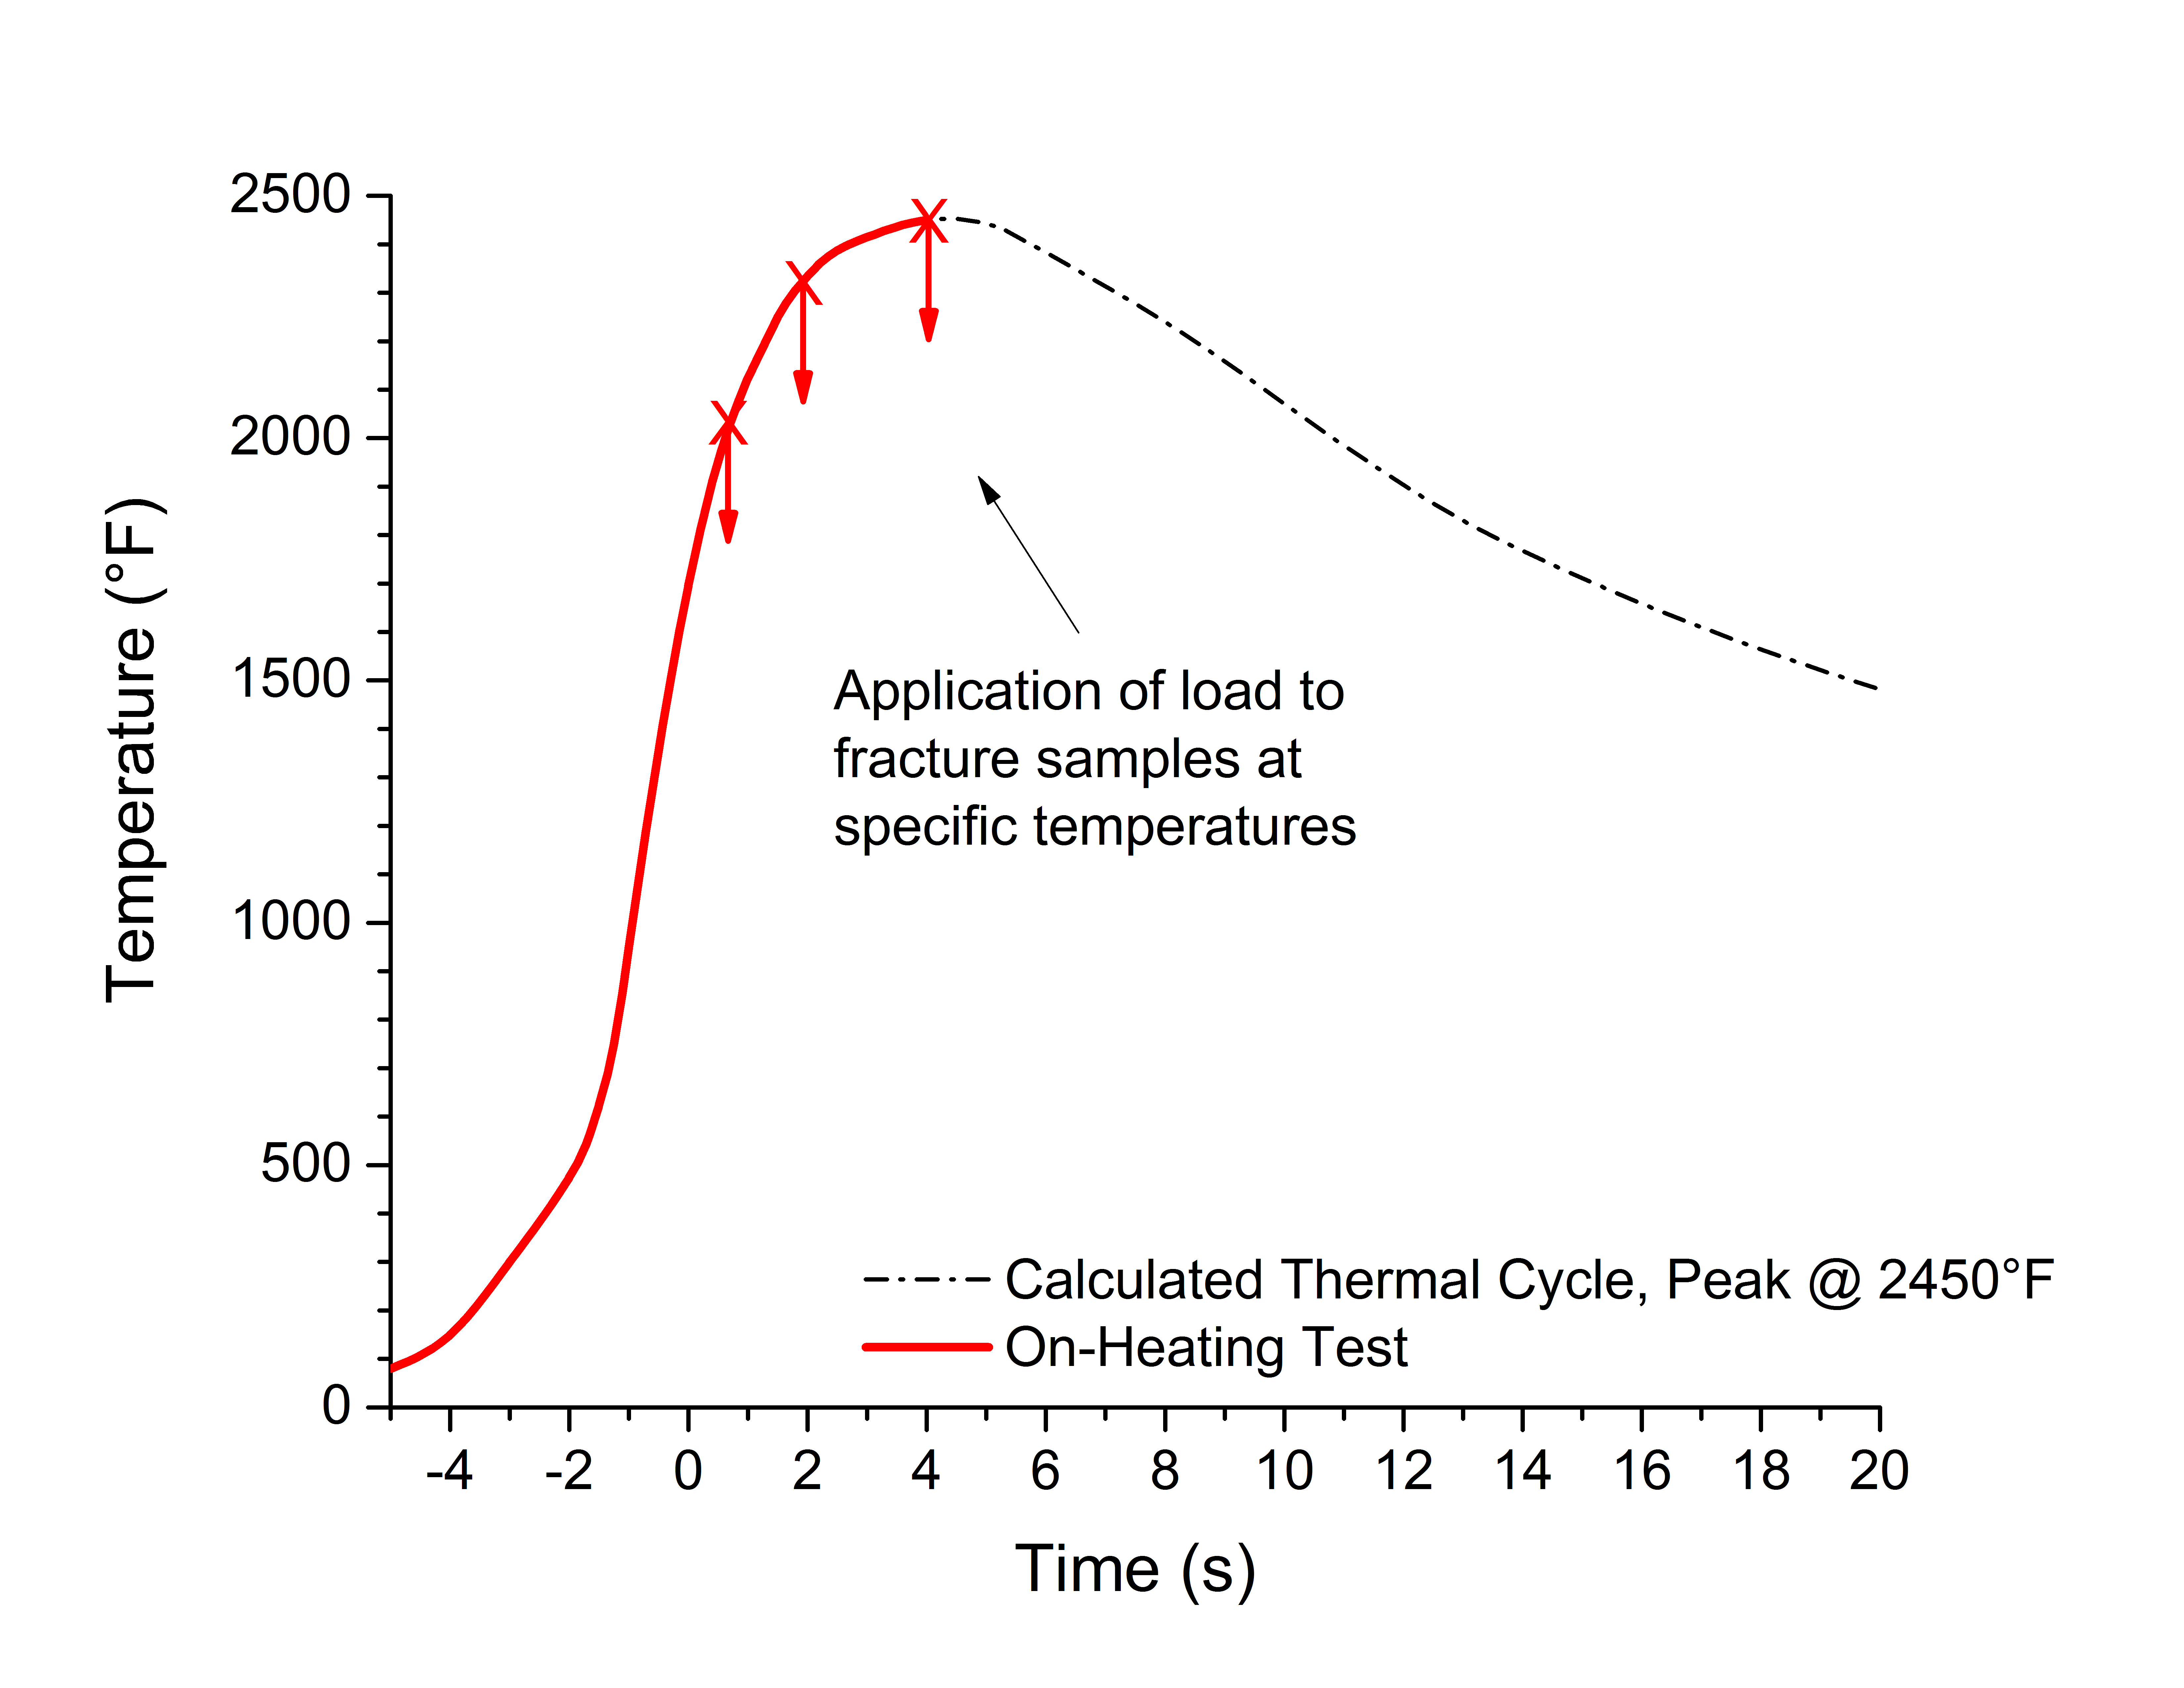
\includegraphics[width=4.5in]{figures/hot-ductility/on-heating-schematic.png}} \\
    \subfloat[On-cooling hot ductility testing]{\label{subfig:on-cooling-schematic}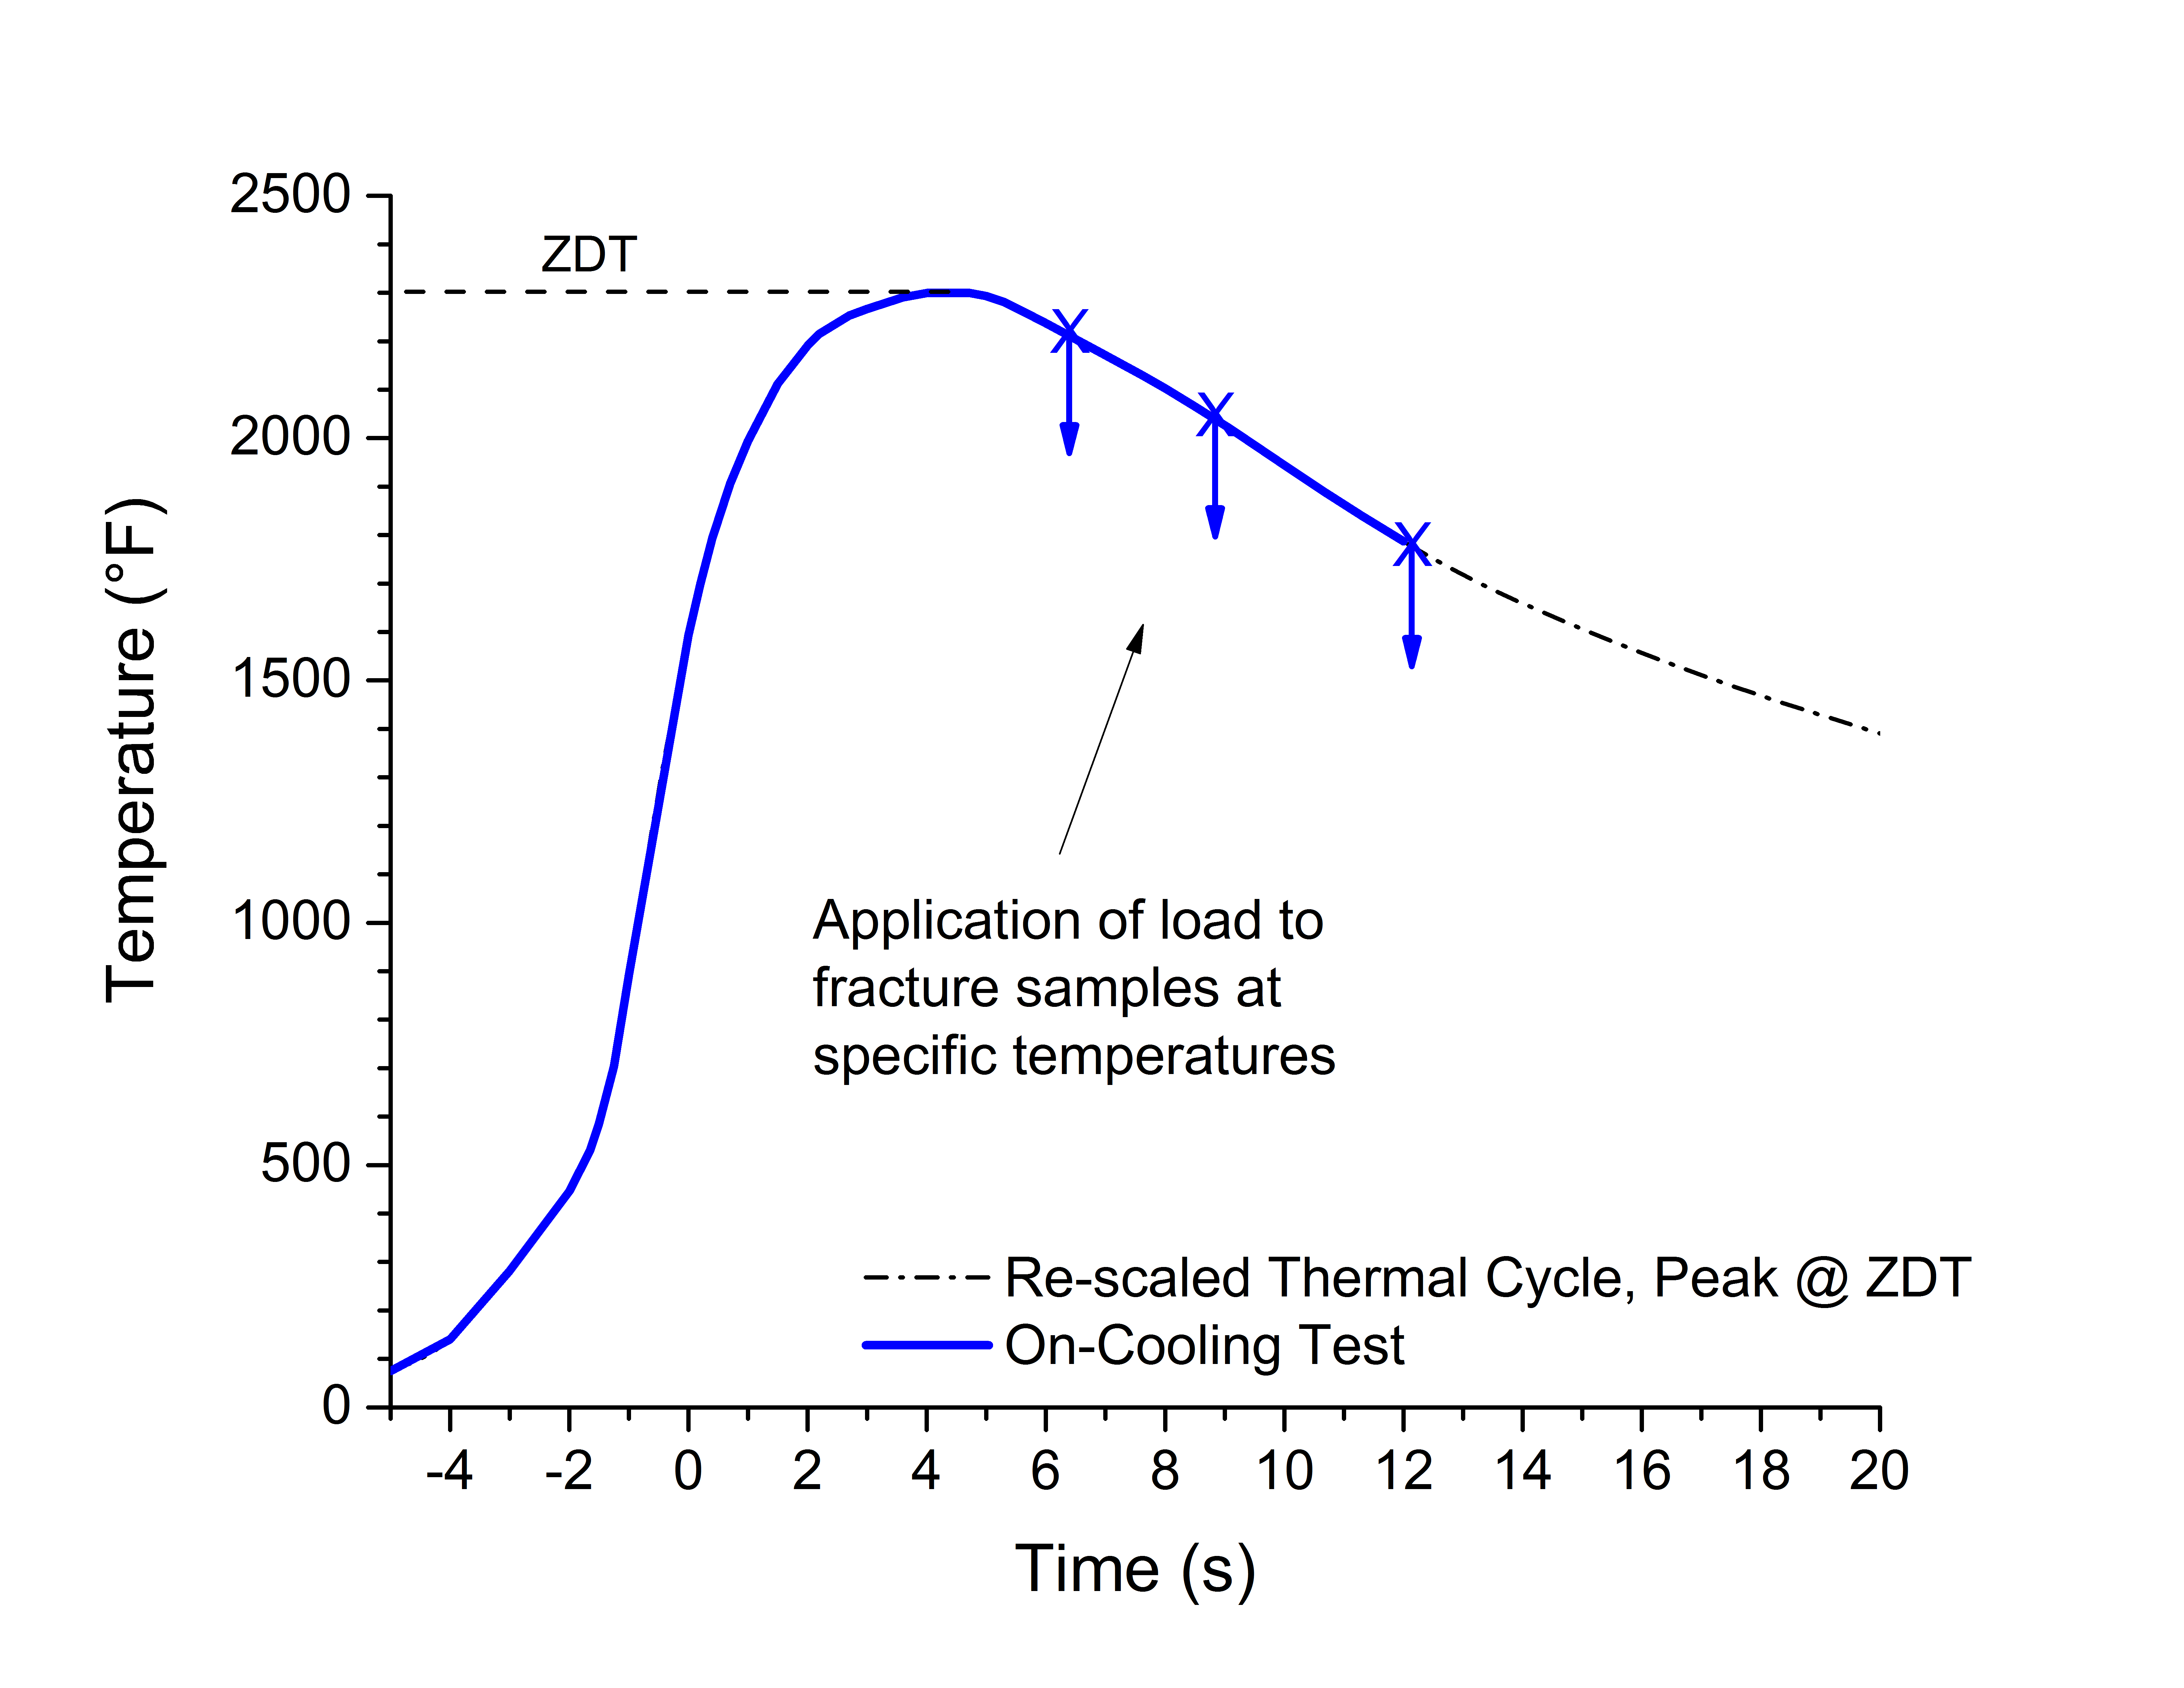
\includegraphics[width=4.5in]{figures/hot-ductility/on-cooling-schematic.png}}
    \caption{Schematic diagrams of on-heating and on-cooling hot ductility tests performed at various temperatures in a simulated welding thermal cycle.}
\end{figure}

\begin{figure}
    \centering
    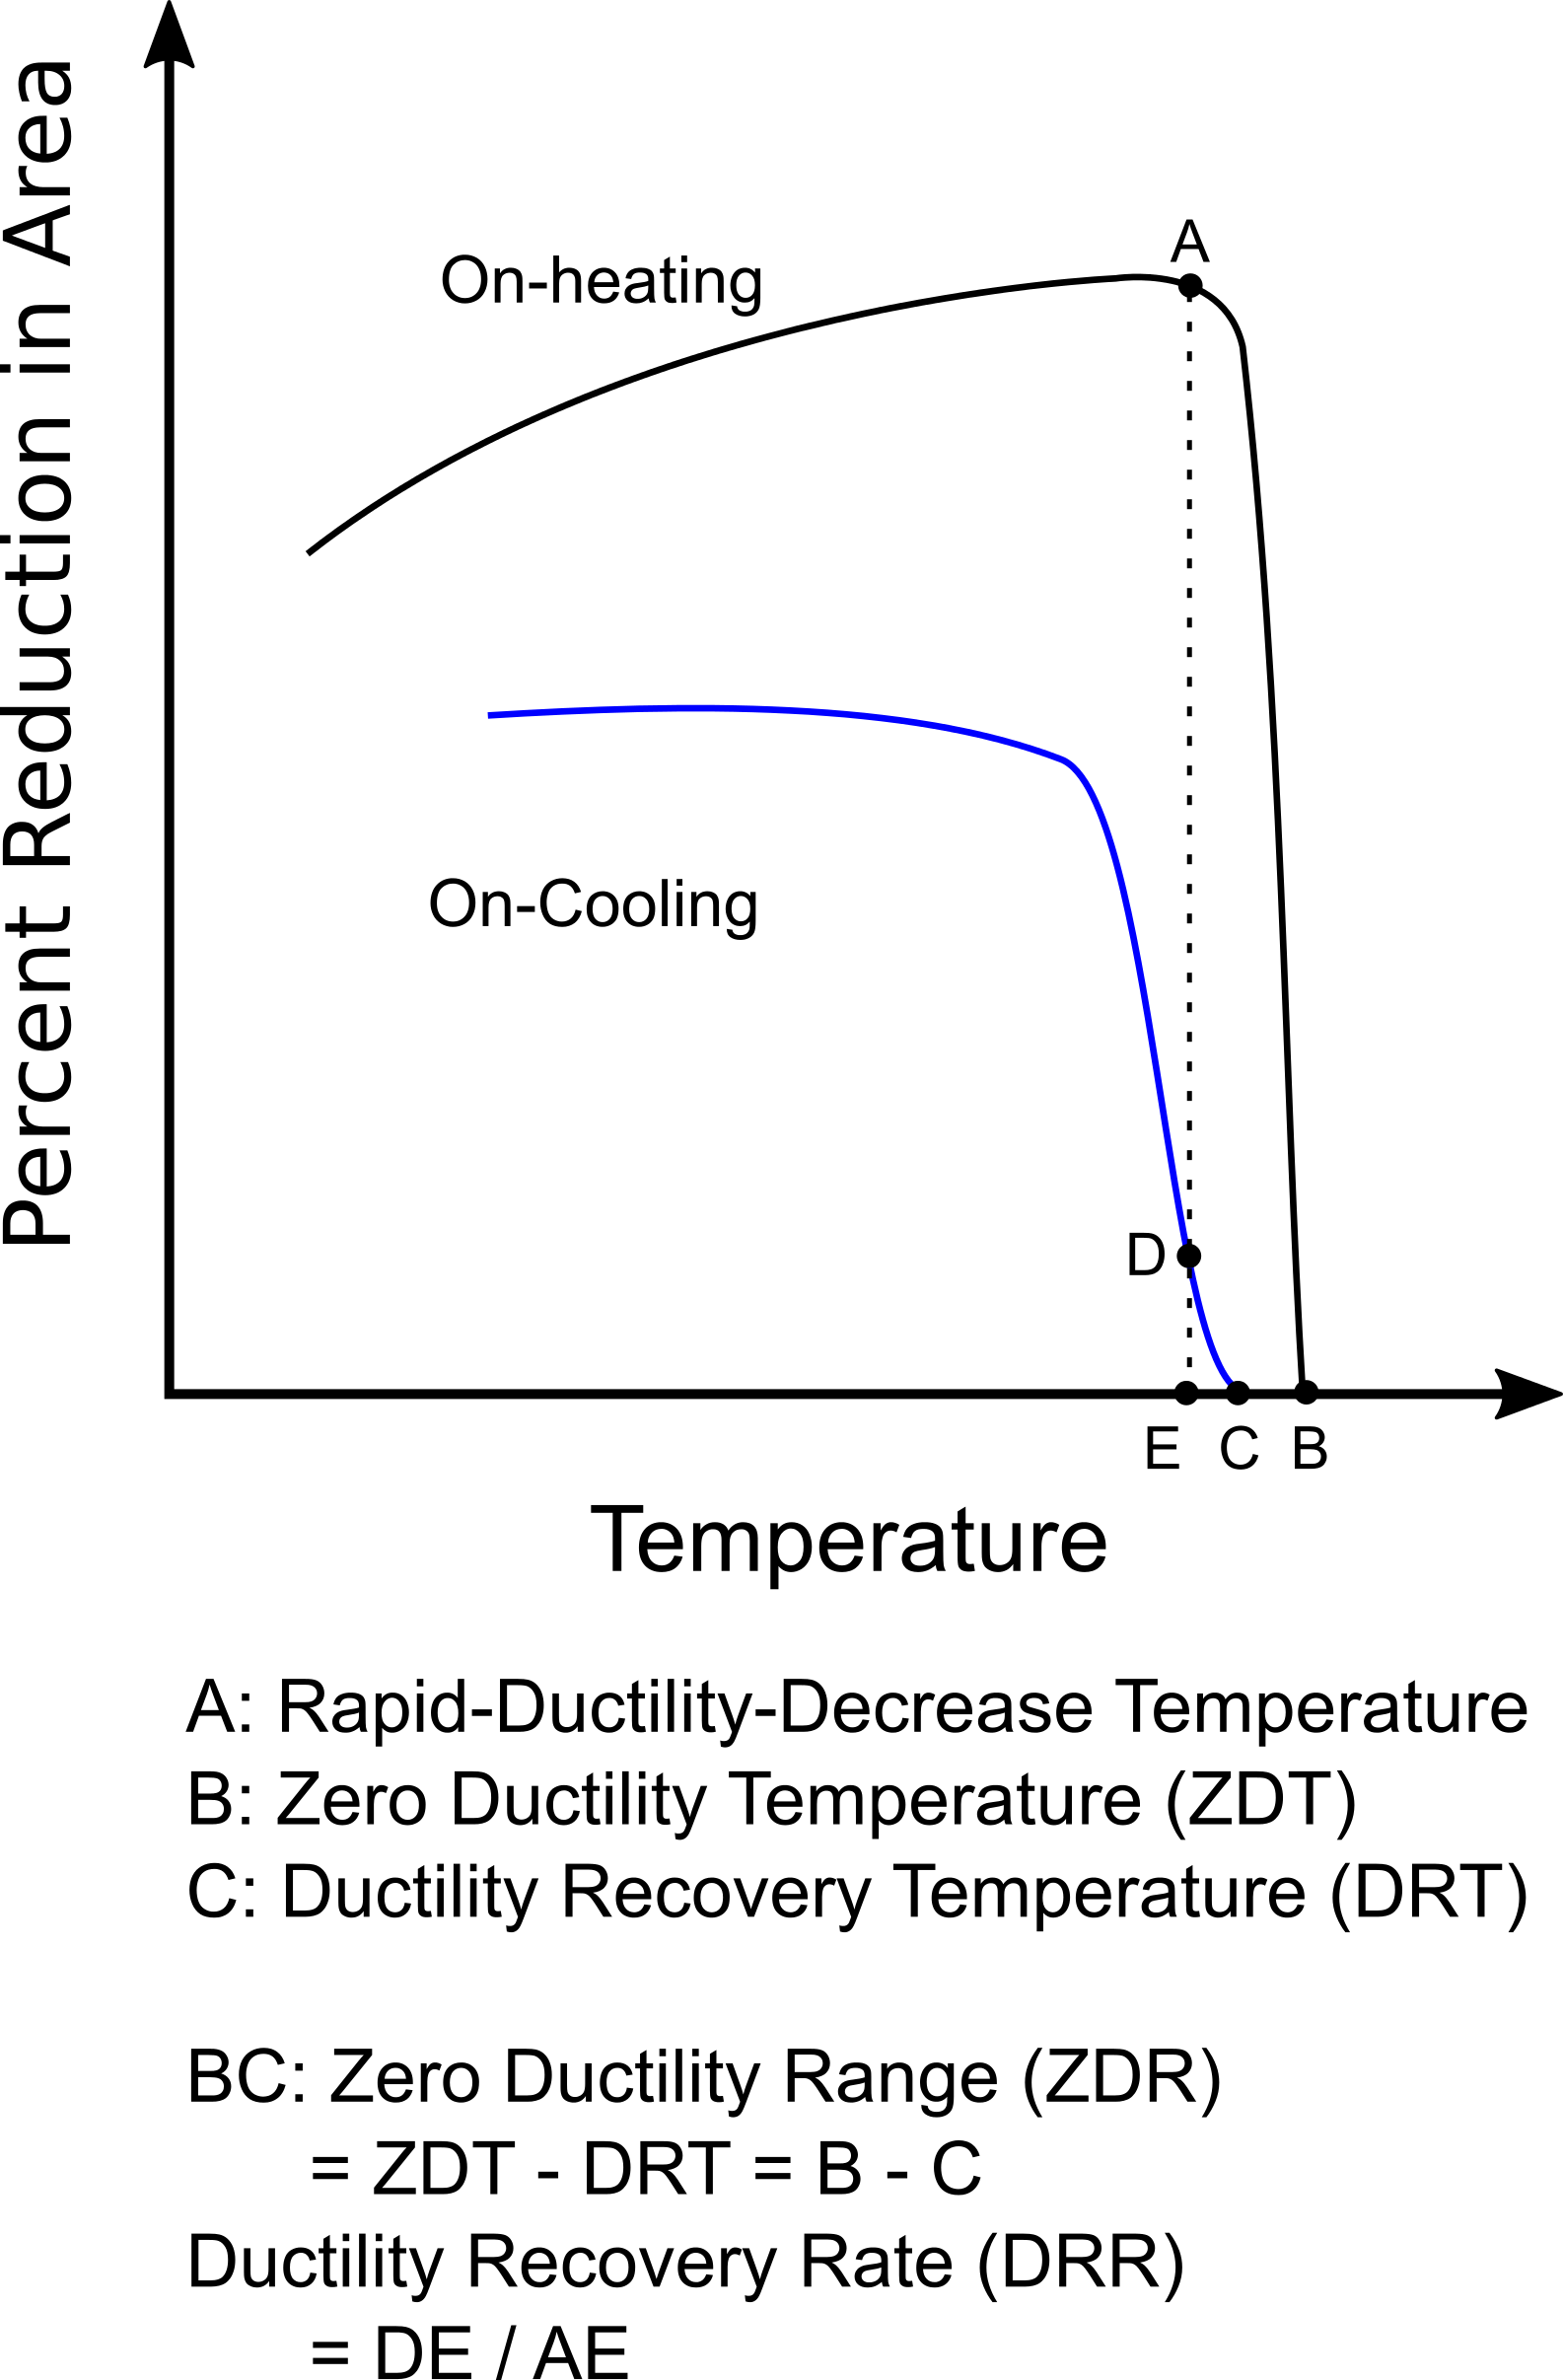
\includegraphics[width=3.5in]{figures/hot-ductility/schematic-hot-ductility-curves.png}
    \caption{Schematic hot ductility curves showing on-heating and on-cooling hot ductility behavior and related evaluation criteria.}
    \label{fig:schematic-hot-ductility-curves}
\end{figure} 
\noindent cited here and to research papers utilizing the Gleeble, can be found in the review articles by~\citet{savage_apparatus_1962},~\citet{lundin_historical_1997}, and~\citet{lundin_standardization_1990_history}. 



\subsection{Hot Ductility Evaluation Criteria}
In one of their early studies utilizing the Gleeble hot ductility test to evaluate a number of alloys, \citet{nippes_further_1957} classified the observed hot ductility responses of the various alloys into several categories, based on the shapes of the hot ductility curves: Classes H1 or H2 for the on-heating behavior and Classes C1, C2, or C3 for the on-cooling behavior. Schematic hot ductility curves illustrating the characteristics of each behavior class are shown in Figure~\ref{fig:nippes-criteria} and a brief text description for each is provided in Table~\ref{tab:nippes-classification}. Of the two on-heating behavior categories, Class H2 (Figure~\ref{fig:nippes-criteria}b) behavior was identified as being intrinsically sensitive to hot cracking. Class H1 behavior (Figure~\ref{fig:nippes-criteria}a) was not considered in and of itself indicative of a propensity for hot cracking and thus required the evaluation of on-cooling results to determine a material's susceptibility. With regard to the on-cooling categories, materials exhibiting Class C1 (Figure~\ref{fig:nippes-criteria}c) behavior were considered not sensitive to hot cracking. Class C2 and Class C3 behaviors (Figure~\ref{fig:nippes-criteria}d,e) were associated with a higher sensitivity to hot cracking, with Class C3 behavior indicating the greatest sensitivity. In particular, \citeauthor{nippes_further_1957} found that those materials in the study which were known to exhibit hot cracking, based on field welding experience, exhibited Class C3 behavior with on-cooling ductility of 40\% or less of the on-heating ductility. Thus, using the Nippes classification system, in most cases a material's on-cooling ductility response will be the major indicating factor regarding its hot cracking susceptibility. Materials exhibiting Class C3 on-cooling behavior with a low recovery of on-cooling ductility (0--40\% of on-heating ductility) can be identified as showing the greatest susceptibility to hot cracking.

Further investigation of hot ductility test criteria was undertaken in a review by \citet{yeniscavich_correlation_1970}. One of the criteria reviewed, attributed to Nippes, was the \gls{drr}. According to this criteria, crack-resistant materials show a rapid recovery of on-cooling ductility after exposure to the \gls{haz} peak temperature, while the on-cooling ductility for crack-sensitive materials recovers slowly and remains low even at test temperatures well below the peak temperature. Schematic curves illustrating the \gls{drr} for crack-resistant and crack-sensitive materials are shown in Figure~\ref{fig:drr-schematic}. Numerically, the \gls{drr} is determined by taking the ratio of the on-cooling ductility to the on-heating ductility at a specified temperature, typically the rapid-ductility-decrease temperature on the on-heating curve (the point on the curve immediately prior to the sudden drop in ductility).


% Nippes Criteria
%\bigskip
\begin{figure}[h]
\centering
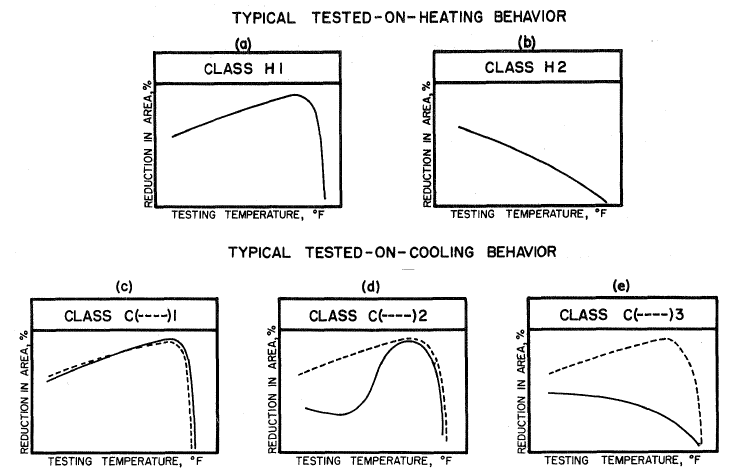
\includegraphics[width=6in]{figures/nippes-criteria.png}
\caption{Classification of hot ductility behavior for on-heating and on-cooling tests; in (c), (d), and (e), the solid line is the on-cooling curve and the dashed line is the on-heating curve.  From \citet[Fig.~66]{nippes_further_1957}.}
\label{fig:nippes-criteria}
\end{figure}

\begin{table}[h]
\caption{Classification of on-heating and on-cooling hot ductility responses based on the work of \citet{nippes_further_1957}. Schematic curves for each behavior class are depicted in Figure~\ref{fig:nippes-criteria}.}
\begin{tabular}{ lp{4in} }
\toprule
\textbf{Classification} & \textbf{Description} \\
\midrule
On-Heating Class H1 & On-heating ductility generally increases as temperature increases, followed by a sudden loss of ductility over a relatively narrow range as the temperature increases further toward the melting point. (Figure~\ref{fig:nippes-criteria}a) \\
\addlinespace
On-Heating Class H2 & On-heating ductility shows a gradual decrease over a wide temperature range as the temperature increases toward the melting point. (Figure~\ref{fig:nippes-criteria}b) \\
& \\
On-Cooling Class C1 & On-cooling ductility is the essentially same as on-heating ductility at all test temperatures. (Figure~\ref{fig:nippes-criteria}c) \\
\addlinespace
On-Cooling Class C2 & On-cooling ductility is the same as on-heating ductility at test temperatures of 2100\textdegree{}F or above, but is significantly lower at test temperatures in the range of 1800--2000\textdegree{}F. (Figure~\ref{fig:nippes-criteria}d) \\
\addlinespace
On-Cooling Class C3 & On-cooling ductility is lower than on-heating ductility at all test temperatures; severity of ductility decrease may change with on-cooling test temperature or with the peak temperature utilized for the on-cooling thermal cycle. (Figure~\ref{fig:nippes-criteria}e) \\
\bottomrule
\end{tabular}
\label{tab:nippes-classification}
\end{table}


\begin{figure}
\centering
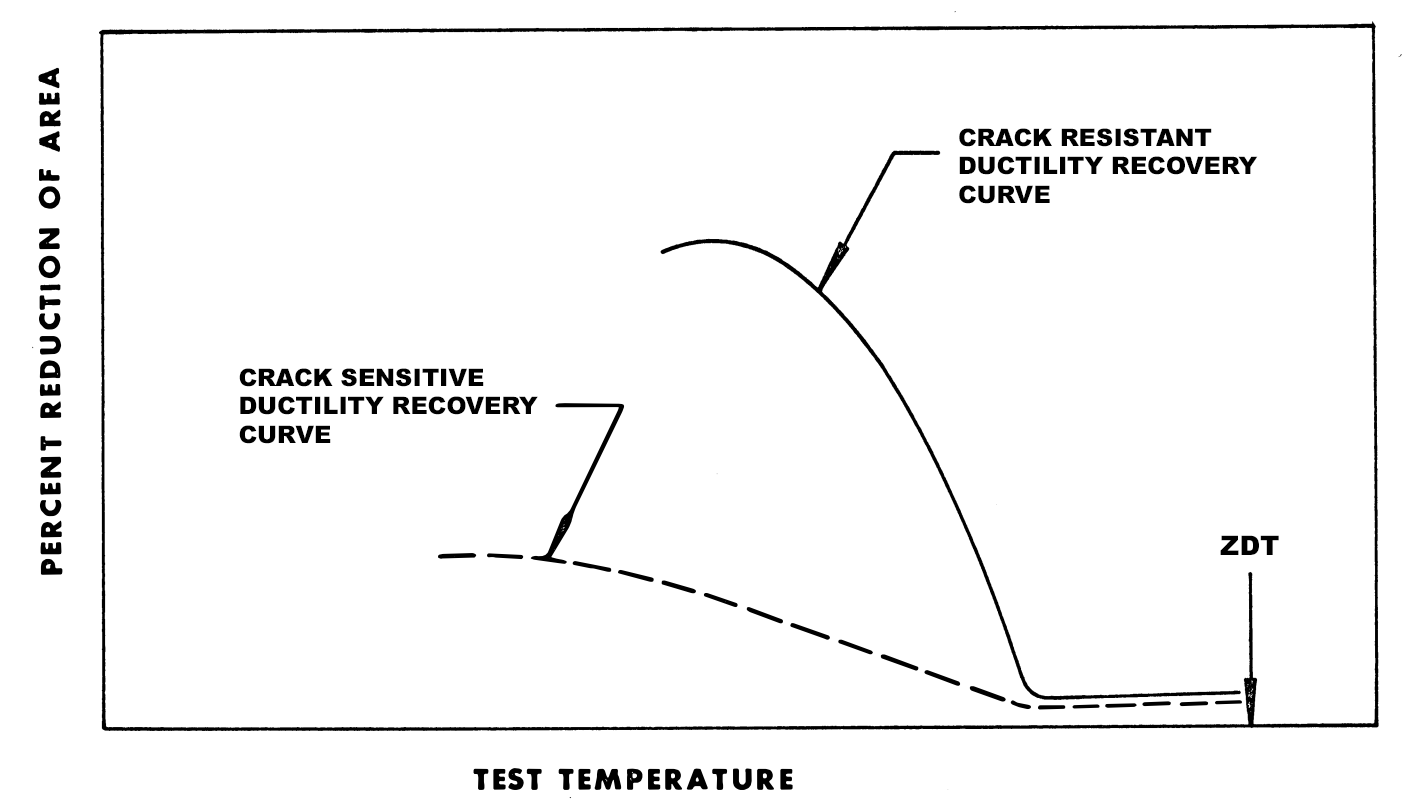
\includegraphics[width=\textwidth]{figures/hot-ductility/DRR-schematic.png}
\caption{Schematic curves illustrating the on-cooling \acrfull{drr} criteria for crack-resistant and crack-sensitive materials.  Adapted from \citet[Fig.~2]{yeniscavich_correlation_1970}}
\label{fig:drr-schematic}
\end{figure}

\citet{yeniscavich_correlation_1970} also proposed the \gls{zdr} as an improved indicator of propensity for hot cracking. The \gls{zdr} phenomenon corresponds to a finite temperature increment below the \gls{zdt} in which the on-cooling ductility remains zero, i.e.~the ductility does not immediately increase once the on-cooling test temperature is below the \gls{zdt}. The physical significance of the \gls{zdr} is related to the fact that the HAZ must possess sufficient ductility to withstand the thermal strains imposed during welding, otherwise cracking will occur. Since the magnitude of these strains is small over the length scale of an HAZ, the HAZ ductility must be on the order of zero for hot cracking to be of concern. Thus, alloys which show a large \gls{zdr} (zero ductility over a wide on-cooling temperature range) are considered more vulnerable to hot cracking than alloys which show a narrow \gls{zdr} (see Figure~\ref{fig:zdr-schematic}).

\begin{figure}
\centering
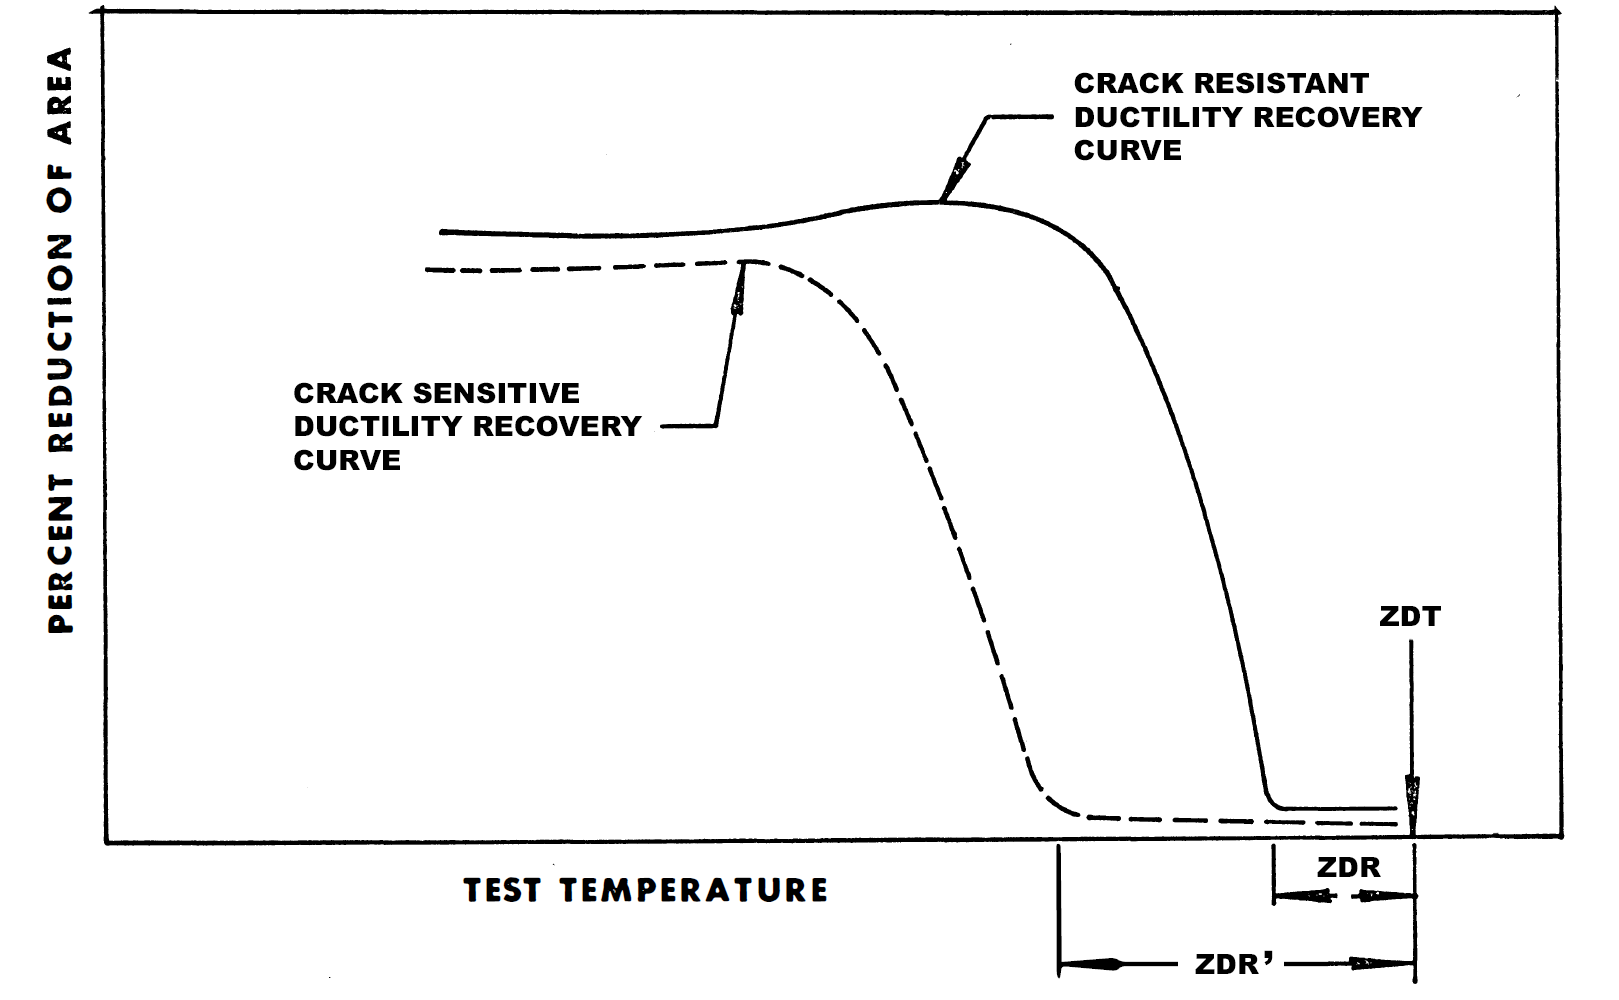
\includegraphics[width=\textwidth]{figures/hot-ductility/zdr-schematic.png}
\caption[Schematic of hot ductility curves illustrating different on-cooling behaviors according to the zero ductility range criteria.]{Schematic of hot ductility curves illustrating different on-cooling behaviors according to the \acrfull{zdr} criteria: crack-sensitive (\gls{zdr}\,\begin{large}{$'$}\end{large} ) and crack-resistant (\gls{zdr}).  Adapted from \citet[Fig.~4]{yeniscavich_correlation_1970}}
\label{fig:zdr-schematic}
\end{figure}


